% %\section{Conceptual Modelling}\label{sec:cm}
% %Conceptually model your database using an E-R diagram. Use the legends in your diagram. Write how you find the entity types, relationships, and attributes from Section~\ref{sec:rga}


% \section{Conceptual Modeling}

% The next step after requirement analysis is conceptual modeling. Conceptual modeling is the process of developing an abstract model or graphical representation using real-world concepts or ideas. It is a high-level diagram that defines, describes, organizes, and presents data elements and their relationships with relatively few details. 

% For this project, the Entity Relationship Model (ERM) was chosen as it is widely used and was emphasized in our course. ERM provides a clear and organized way to represent data structures, which is essential for the campus event management system.

% \subsection{Entity-Relationship Model}

% An Entity-Relationship Diagram (ERD) shows the relationships of entities stored in a database. ER diagrams explain the logical structure of a database and illustrate how entities interact. In ER diagrams, three basic concepts are used:

% \begin{enumerate}
%     \item \textbf{Entity}: In database management systems, an entity is a data object that represents a real-world object or concept, such as an event or a participant. Entities are often represented as tables, with each row representing a specific instance. Entities are shown in rectangular shapes in the ER model.

%     \item \textbf{Attribute}: An attribute represents a characteristic or property of an entity. For example, attributes for an event entity might include \textit{event name}, \textit{date}, and \textit{location}. Attributes are represented by oval shapes in the ER model.

%     \item \textbf{Relationship}: Relationships are connections between entities that define how data in one entity relates to data in another. In the ER diagram, relationships between entities are represented by diamonds and are labeled to describe the interaction. Common types of relationships include:
%     \begin{enumerate}
%         \item One-to-One
%         \item One-to-Many
%         \item Many-to-One
%         \item Many-to-Many
%     \end{enumerate}
% \end{enumerate}

% \subsection{Detailing the Entity-Relationship Model}

% From the analysis, the following entities and relationships have been identified for the Campus Event Management System:

% \subsubsection{Entity Types}

% \begin{enumerate}
%     \item \textbf{User}: Represents users of the system with attributes such as \textit{user\_id}, \textit{username}, \textit{email}, \textit{password}, \textit{user\_type}, \textit{created\_at}, \textit{last\_login},and \textit{contact\_number}.
%     \item \textbf{Event}: Represents each campus event, including attributes like \textit{event\_id}, \textit{event\_name}, \textit{description}, \textit{event\_date}, \textit{start\_time}, \textit{end\_time}, \textit{location\_id}, \textit{organizer\_id}, \textit{status}, and \textit{max\_attendees}.
    
%     % adding teacher and student
%     \item \textbf{Teacher}: Represents faculty members involved in events, including attributes like \textit{teacher\_id}, \textit{name}, \textit{email}, \textit{department}, \textit{phone\_number}, and \textit{user\_id}.
    
%     \item \textbf{Student}: Represents students who may attend events, including attributes like \textit{student\_id}, \textit{name}, \textit{email}, \textit{enrollment\_year}, \textit{major}, and \textit{user\_id}.
    
%     \item \textbf{Organizer}: Represents individuals organizing events with attributes such as \textit{organizer\_id}, \textit{name}, \textit{contact\_number}, \textit{email}, \textit{user\_id}, and \textit{organization}.
%     % \item \textbf{Participant}: Represents people attending events, including attributes like \textit{participant\_id}, \textit{event\_id}, \textit{user\_id}, \textit{registration\_date}, and \textit{status}.
%     \item \textbf{Location}: Represents locations where events are held, with attributes like \textit{location\_id}, \textit{room\_name}, \textit{building}, \textit{capacity}, and \textit{availability\_status}.
%     % \item \textbf{Resource}: Represents resources allocated for events, including attributes like \textit{resource\_id}, \textit{resource\_type}, \textit{quantity}, \textit{availability\_status}, and \textit{location\_id}.
%     % \item \textbf{Booking}: Represents the booking of locations and resources, with attributes like \textit{booking\_id}, \textit{event\_id}, \textit{location\_id}, \textit{resource\_id}, \textit{start\_time}, and \textit{end\_time}.
%     % \item \textbf{Notification}: Represents notifications sent to users with attributes like \textit{notification\_id}, \textit{user\_id}, \textit{event\_id}, \textit{message}, \textit{notification\_date}, and \textit{status}.
% \end{enumerate}

% \subsubsection{Relationship Types}

% The relationships between the entities identified in the ER model are as follows:

% \begin{itemize}
%     \item \textbf{Organized by}: Connects \textit{Organizer} and \textit{Event} entities, where each organizer can manage multiple events.
%     \item \textbf{Registers}: Connects \textit{Participant} and \textit{Event} entities, where a participant can register for multiple events, and each event can have multiple participants.
%     % \item \textbf{Requires}: Connects \textit{Event} and \textit{Resource} entities, where an event may require multiple resources, and each resource can be allocated to multiple events.
%     \item \textbf{Located At}: Connects \textit{Event} and \textit{Location} entities, where each event is held in a specified location.
% \end{itemize}
% \begin{figure}[h]
%     \centering
%     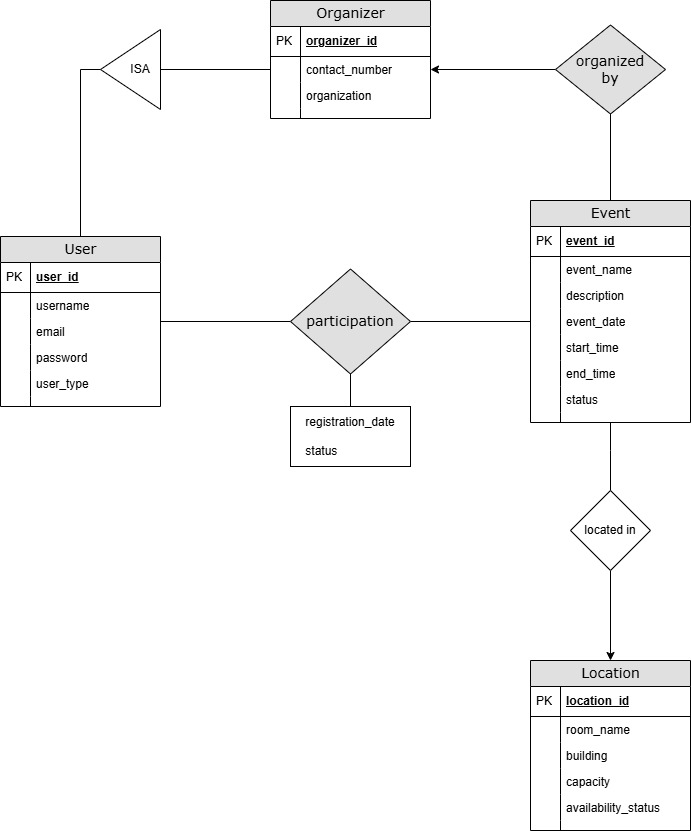
\includegraphics[scale=0.4]{images/Event_Management2.jpg}
% \end{figure}
% In the figure the ER diagram displays these entity types and their relationships. For instance, the relationship between \textbf{Event} and \textbf{Participant} indicates that one participant can register for multiple events. The \textbf{Organizer} manages one or more events, and resources are allocated to events as needed.

% Entities are represented in rectangular shapes, relationships in diamond shapes, and attributes in oval shapes.


\section{Conceptual Model for Campus Event Management System}

The conceptual model for the Campus Event Management System was developed using the Entity-Relationship Model (ERM). The ERM was chosen because of its clarity in representing data structures and its relevance to our coursework. ER diagrams define the logical structure of the database, showing how data elements and their relationships interact within the system.

\subsection{Entity-Relationship Model}

An \textbf{Entity-Relationship Diagram (ERD)} visually represents the data structure of the Campus Event Management System, showing how entities and their attributes relate to each other.

\textbf{Key Concepts in the ER Model:}

\begin{itemize}
    \item \textbf{Entity}: An entity represents a real-world object or concept, like an event or user. Entities are represented as tables in the database, with each row representing a specific instance.
    \item \textbf{Attribute}: Attributes represent the properties or characteristics of an entity. For example, attributes of the \texttt{Event} entity include \texttt{event\_name}, \texttt{event\_date}, and \texttt{location\_id}.
    \item \textbf{Relationship}: Relationships define the interactions between entities. Common types of relationships include:
    \begin{itemize}
        \item \textbf{One-to-One}
        \item \textbf{One-to-Many}
        \item \textbf{Many-to-One}
        \item \textbf{Many-to-Many}
    \end{itemize}
\end{itemize}

\subsection{Detailing the Entity-Relationship Model}

From the analysis, the following \textbf{entities} and \textbf{relationships} have been identified for the Campus Event Management System.

\subsubsection{Entity Types}

\begin{enumerate}
    \item \textbf{User}: Represents users of the system with attributes:
    \begin{itemize}
        \item \texttt{username} (Primary Key)
        \item \texttt{name}
        \item \texttt{email}
        \item \texttt{password}
        \item \texttt{user\_type} (enum: `student`, `teacher`)
        \item \texttt{contact\_number}
    \end{itemize}

    \item \textbf{Student}: Represents students who may attend events, with attributes:
    \begin{itemize}
        \item \texttt{student\_id} (Primary Key)
        \item \texttt{enrollment\_date}
        \item \texttt{username} (Foreign Key referencing \texttt{User.username})

    \end{itemize}

    \item \textbf{Teacher}: Represents faculty members involved in events, with attributes:
    \begin{itemize}
        \item \texttt{teacher\_id} (Primary Key)
        \item \texttt{employment\_date}
        \item \texttt{username} (Foreign Key referencing \texttt{User.username})
    \end{itemize}

    \item \textbf{Event}: Represents each campus event, with attributes:
    \begin{itemize}
        \item \texttt{event\_id} (Primary Key)
        \item \texttt{event\_name}
        \item \texttt{description}
        \item \texttt{event\_date}
        \item \texttt{start\_time}
        \item \texttt{end\_time}
        \item \texttt{status} (enum: `pending`, `ongoing`, `finished`)
        \item \texttt{max\_attendees}
        
        \item \texttt{category\_id} (Foreign Key referencing \texttt{Event\_Category.category\_id})
        \item \texttt{location\_id} (Foreign Key referencing \texttt{Location.location\_id})
    \end{itemize}

    \item \textbf{Location}: Represents locations of the venues:
    \begin{itemize}
        \item \texttt{location\_id} (Primary Key)
        \item \texttt{location\_name}
    \end{itemize}

    \item \textbf{Venue}: Represents locations where events are held, with attributes:
    \begin{itemize}
        \item \texttt{venue\_id} (Primary Key)
        \item \texttt{venue\_name}
        \item \texttt{location\_id} (Foreign Key referencing \texttt{Location.location\_id})
    \end{itemize}

    
    \item \textbf{Event Category}: Represents categories for events, with attributes:
    \begin{itemize}
        \item \texttt{category\_id} (Primary Key)
        \item \texttt{category\_name}
    \end{itemize}
\end{enumerate}

\subsubsection{Relationship Types}

The relationships between the entities are as follows:

\begin{itemize}
    \item \textbf{Organized\_By}: Connects \texttt{User} and \texttt{Event}, where each user (acting as an organizer) can manage multiple events.
    \begin{itemize}
        \item \texttt{username} (Foreign Key referencing \texttt{User.username})
        \item \texttt{event\_id} (Foreign Key referencing \texttt{Event.event\_id})
    \end{itemize}

    \item \textbf{Registers}: Connects \texttt{User} (as a participant) and \texttt{Event}, where a participant can register for multiple events, and each event can have multiple participants.
    \begin{itemize}
        \item \texttt{username} (Foreign Key referencing \texttt{User.username})
        \item \texttt{event\_id} (Foreign Key referencing \texttt{Event.event\_id})
        \item \texttt{registration\_date}
    \end{itemize}

    \item \textbf{held At}: Connects \texttt{Event} and \texttt{Venue}, where each event is held at a specified venue.
    \begin{itemize}
        \item \texttt{venue\_id} (Foreign Key referencing \texttt{Venue.venue\_id})
        \item \texttt{event\_id} (Foreign Key referencing \texttt{Event.event\_id})
    \end{itemize}
    \item \textbf{located in}: Connects \texttt{Venue} and \texttt{Location}, where each venue is located in a specified location.
    \begin{itemize}
        \item \texttt{venue\_id} (Foreign Key referencing \texttt{Venue.venue\_id})
        \item \texttt{location\_id} (Foreign Key referencing \texttt{Location.location\_id})
    \end{itemize}
\end{itemize}
\newpage
\begin{figure}[h]
    \centering
    \vspace{-1cm}
    \hspace*{-3cm} % Adjust this value for the desired left margin
    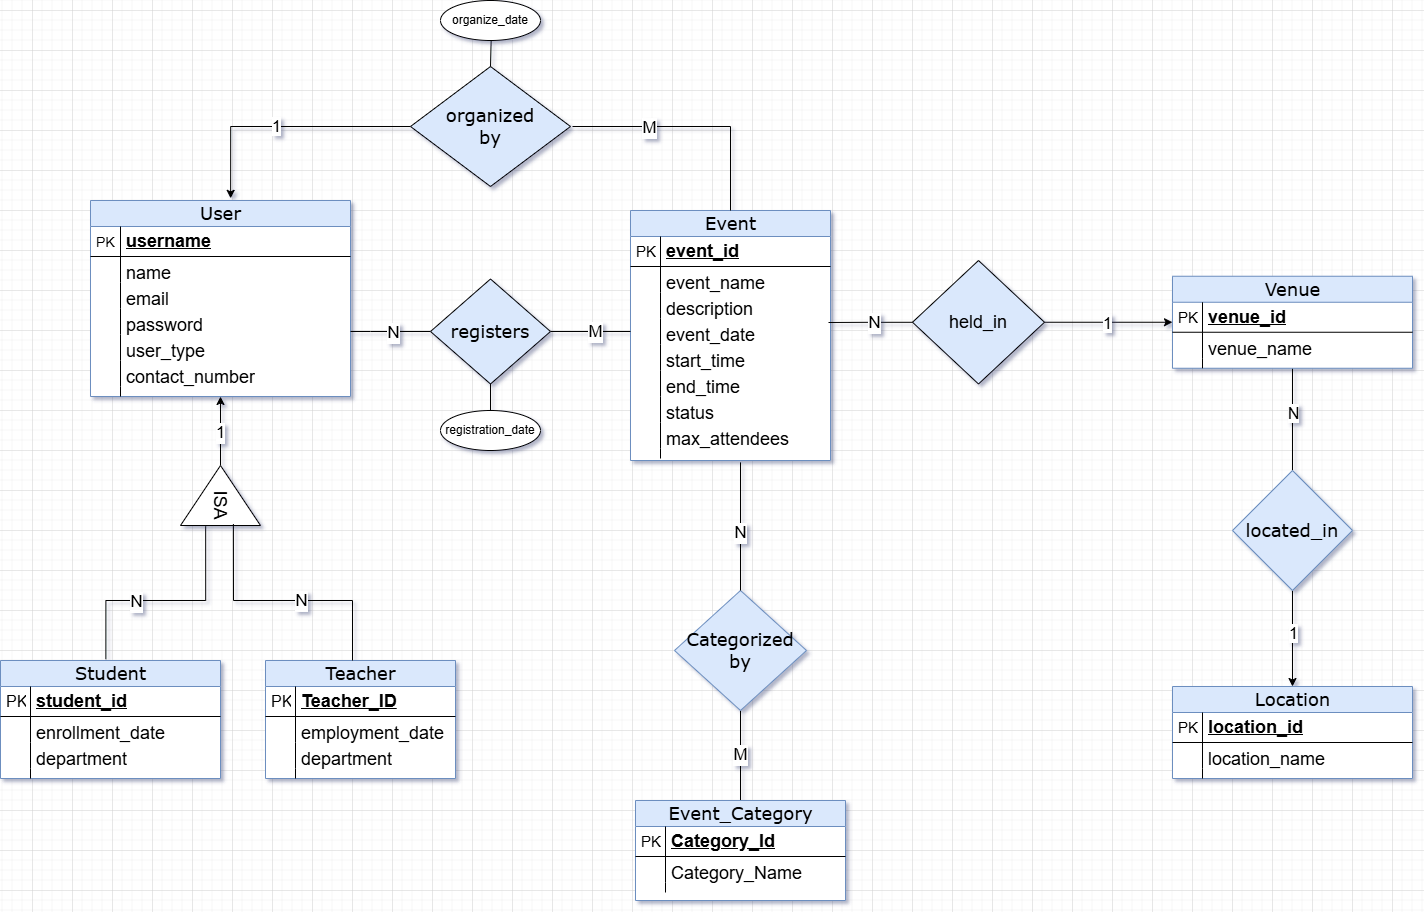
\includegraphics[scale=.4]{images/meetup2.0.drawio.png}
\end{figure}


This ER model provides a high-level structure for managing campus events, representing how data is organized within the Campus Event Management System. The relationships between entities allow efficient linking of users, events, locations, and categories, facilitating seamless interactions within the system.
\clearpage